The system was implemented in \textit{C++} with interface with ROS. The design (Fig.~\ref{fig:system_architecture}) was created following the description done in previous sections. 
\begin{figure*}
	\centering
	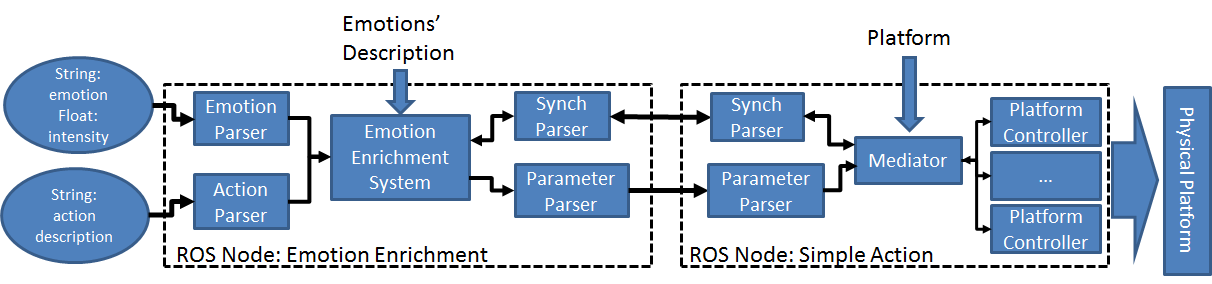
\includegraphics[width=1.0\textwidth]{Images/SystemArchitecture.png} 	
	\caption{General system design. Each simple action corresponds to one ROS node, and there is just one node for the emotion enrichment system. The ovals represent the ROS topic parameters, rectangles represent \textit{black boxes}, and texts outside containers represent input files that contain the system parametrization.}
	\label{fig:system_architecture}
\end{figure*}
The emotion enrichment core is divided in three different modules. 
Each module is responsible for one of the following phases:
\begin{enumerate}
	\item \textit{Generation of emotional execution tree:} this phase starts every time that a new action message is received. The process begins by parsing the format, verifying that the actions described on it exist in the system, and that the parameters correspond to the ones expected by each action described on the message. This parameters' verification is done on the implemented description for each action, which describes the parameters that are mandatory and those that are optional. When the verification is done, and all the action exists and  the parameters correspond, an $ext$ is created such as the one presented in the Figure~\ref{fig:reference} that corresponds to the example of walk and speak.
	\begin{figure}
		\centering
		%Representation
	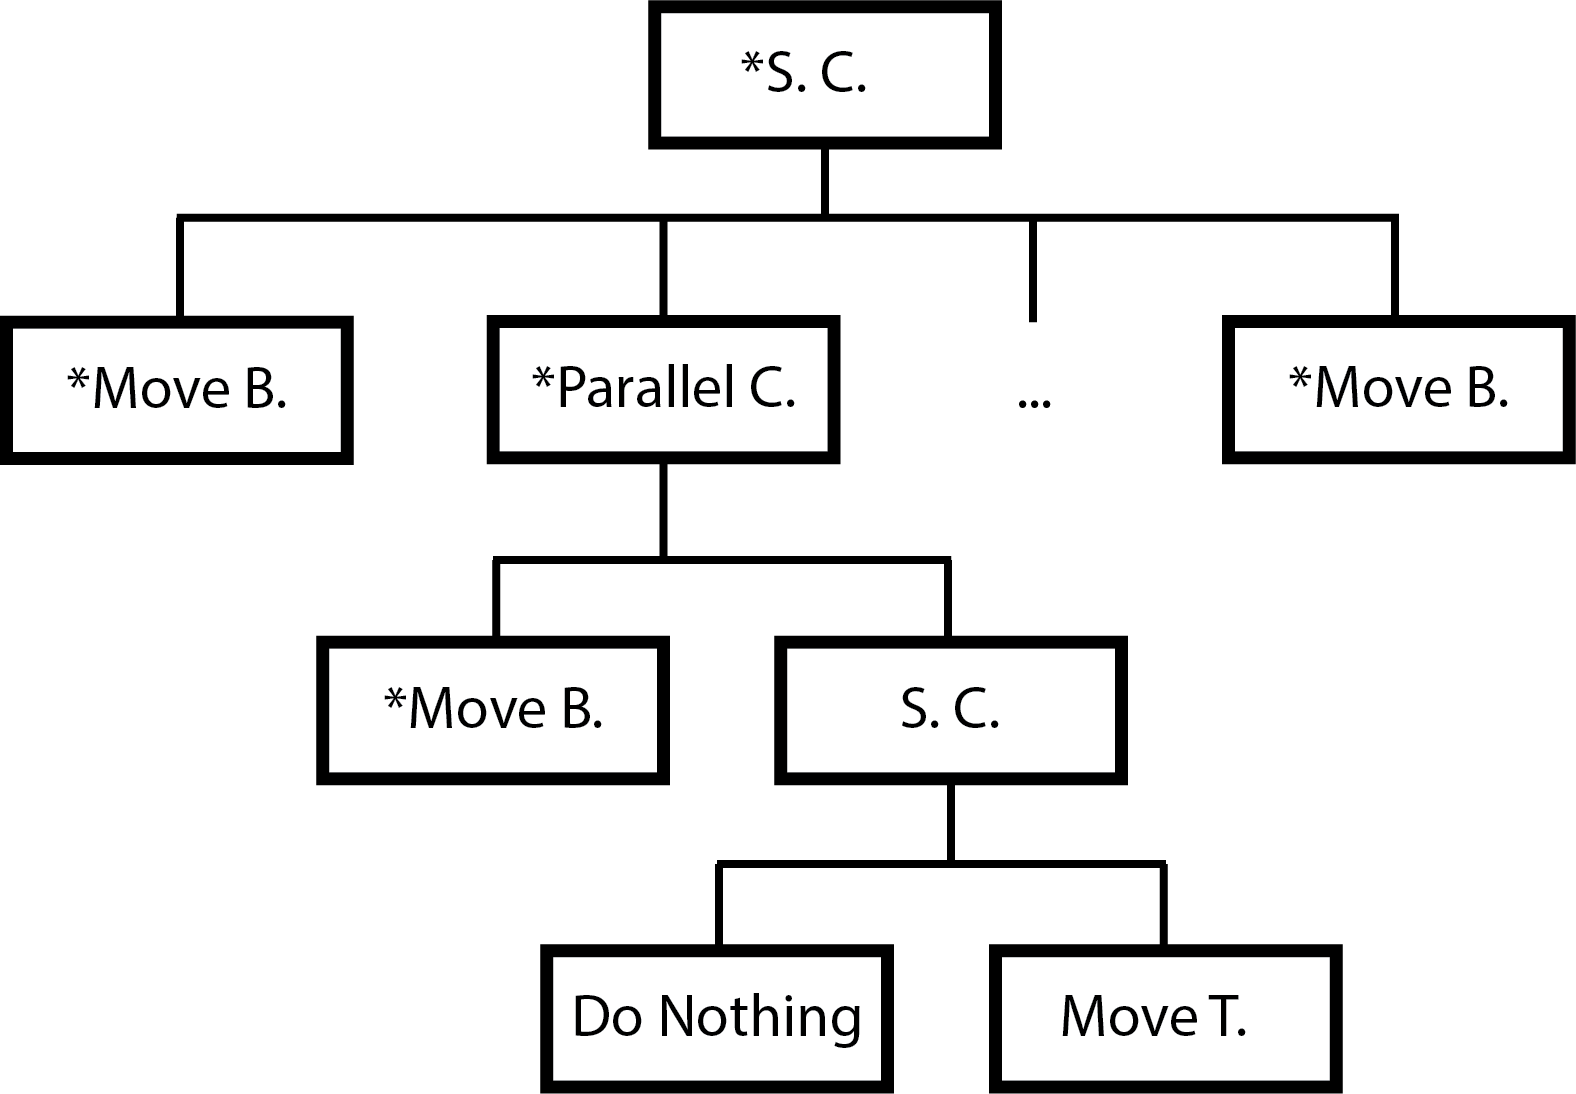
\includegraphics[width=0.45\textwidth]{./Images/Representation.png}
	\caption{Emotional Execution Tree for the example shown in the Figure~\ref{fig:compound_example}. The context node colored in purple represents a sequential context, while the other represents a parallel.}
	\label{fig:reference}
	\end{figure}
	\item \textit{Emotion addition:} uses the $ext$ created in the previous phase. In this phase new $sa$ are added to the $ext$ and the $sa$'s parameters are modified following the emotion description, which is loaded from files. This process is broken down in two steps. First, all the actions that are required to convey the desired emotion, and that are not yet present are added. Second, the emotional parameters are modulated based on the emotion's intensity and character traits.
	\item \textit{Execution:} this is the last phase and it is done after the $ext$ is ''coloured'' with emotional characteristics (actions additions and emotional parameters). The decision to have two different communication channels, one for action parameters and another for the action emotional parameters, was taken to enable the possibility to update the emotional parameters without interfering with the current execution. In this phase is maintain a reference to the mandatory and emotional action, thus when a new emotion is received the system stops the previous emotional action and start executing the new ones without affecting the general execution of the actions.
\end{enumerate}
%The first one is in charge to receive any action and built a $EXT$. Once this tree is created, the second part is in charge to decorate this tree with the additional actions and modify the parameters of all the actions. The last part is the one that executes the final tree and communicate to all the simple actions ROS nodes the parameters that should be executed by them. It is important to notice that the action's parameters and the emotional parameters are communicated via two different channels. This is done to not affect actions' execution when the emotion or its intensity is changed.
All the text message broadcast among the nodes are written using JSON format, which is human understandable, is light and there are diverse available parser.\\ 
To test the system was used to different platforms: Keepon Pro and an own made platform called Triskarino.
Keepon was used to test the interoperability of the system to different platforms, while Triskarino has been used as a part of the robot actor project~\cite{angel2013}. The whole TheatreBot architecture has not finished just, thus the change of emotion and selection of action to execute were done manually.
%%%%%%%%%%%%%%%%%%%%%%%%%
%%%%%%%%%%%%%%%%%%%%%%%%%%%%%
\subsection{Keepon Test}
To test the system with Keepon (Fig.~\ref{fig:keepon}) was just necessary to implement the platform's controllers in each one of the simple action ROS nodes. Given that this platform does not have the capability to displace its body, the action move body was not implemented. Once added these controllers to the system, we proceeded to modify the configuration files to use this platform instead of Triskarino. With this small modification, we were able to change from one platform to other. In the video\footnote{YouTube video name Emotional Enrichment System, url: https://youtu.be/bRSXQ0rzkO8}
 is shown the test where Keepon has to move its torso forward and backward with a ``happy'' emotion. 
\begin{figure}
	\centering
	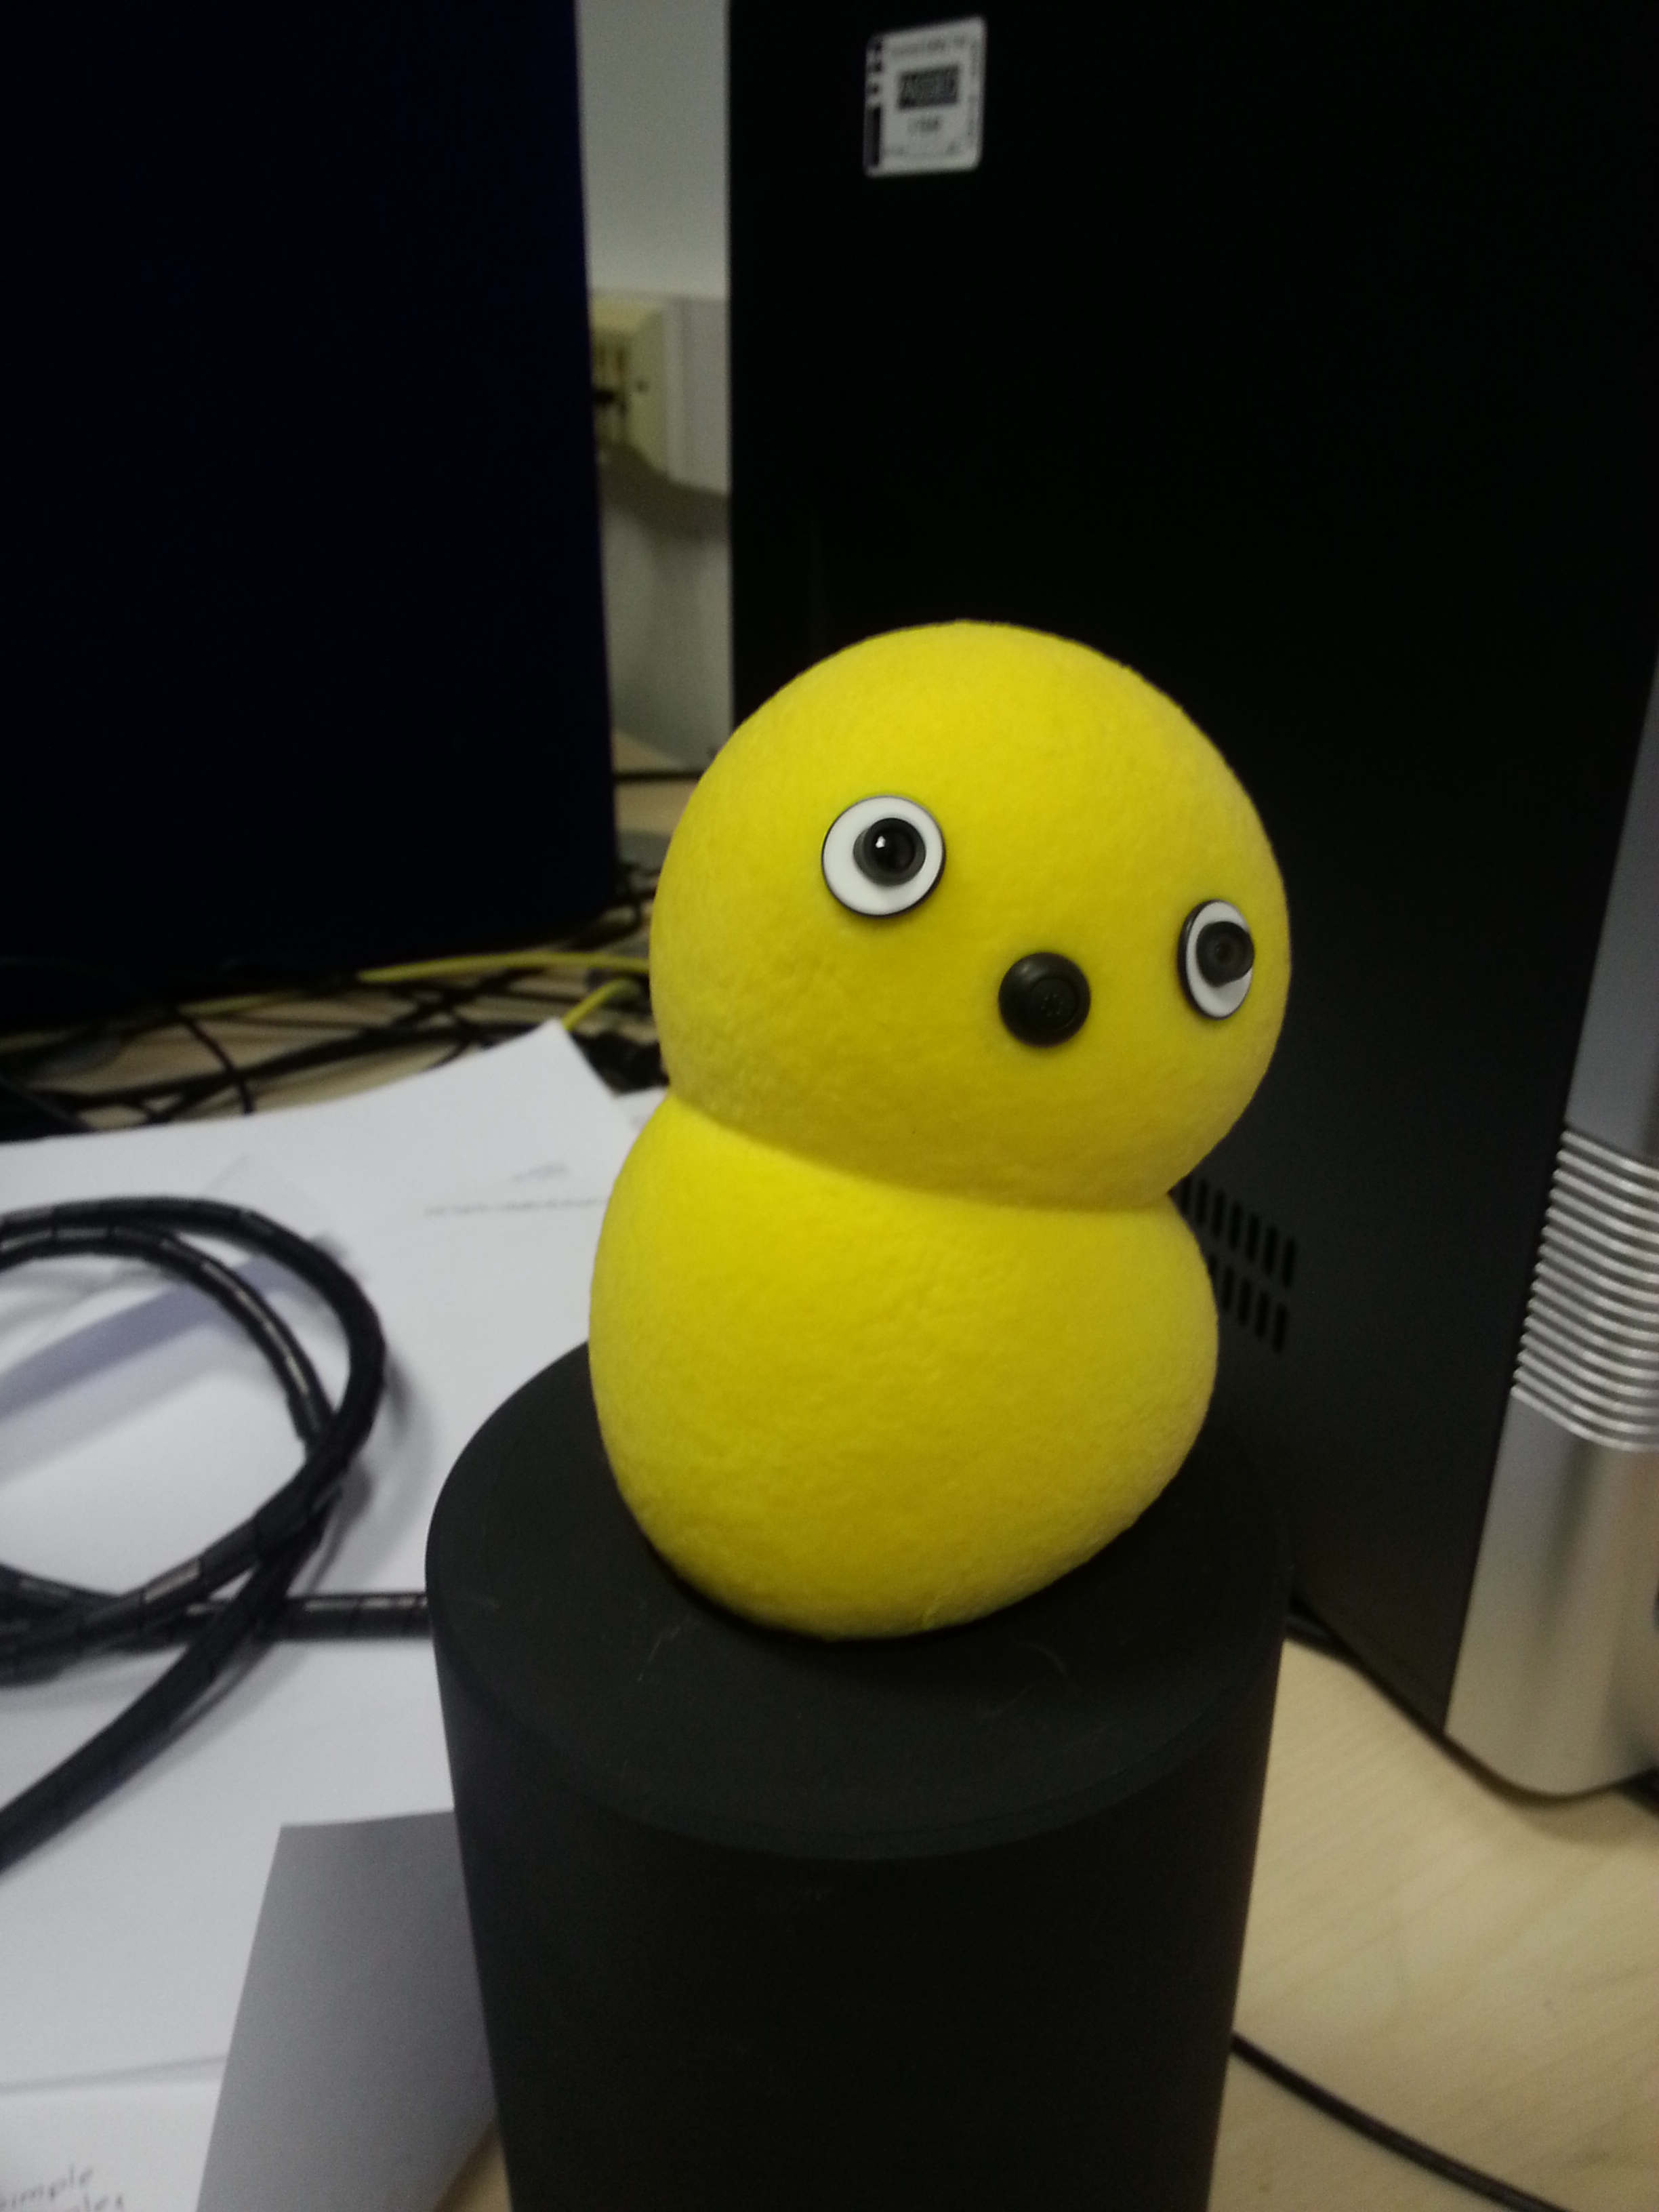
\includegraphics[width=0.2\textwidth]{./Images/Keepon.jpg}
	\caption{Keepon platform.}
	\label{fig:keepon}
\end{figure} 
 The action is given by a console telling the robot to bend the torso to a desire angle in x. The torso oscillation in y is added automatically by the system following the description given to happiness. 
 %%%%%%%%%%%%%%%%%%%%%
%%%%%%%%%%%%%%%%%%%%%%%%%%%%%
\subsection{Triskarino Test}
 The system has been widely used with Triskarino (Fig.~\ref{fig:robot}) during our studies on projecting emotions with a non human like platform. 
\begin{figure}
	\centering
	\begin{subfigure}[c]{0.2\textwidth}
	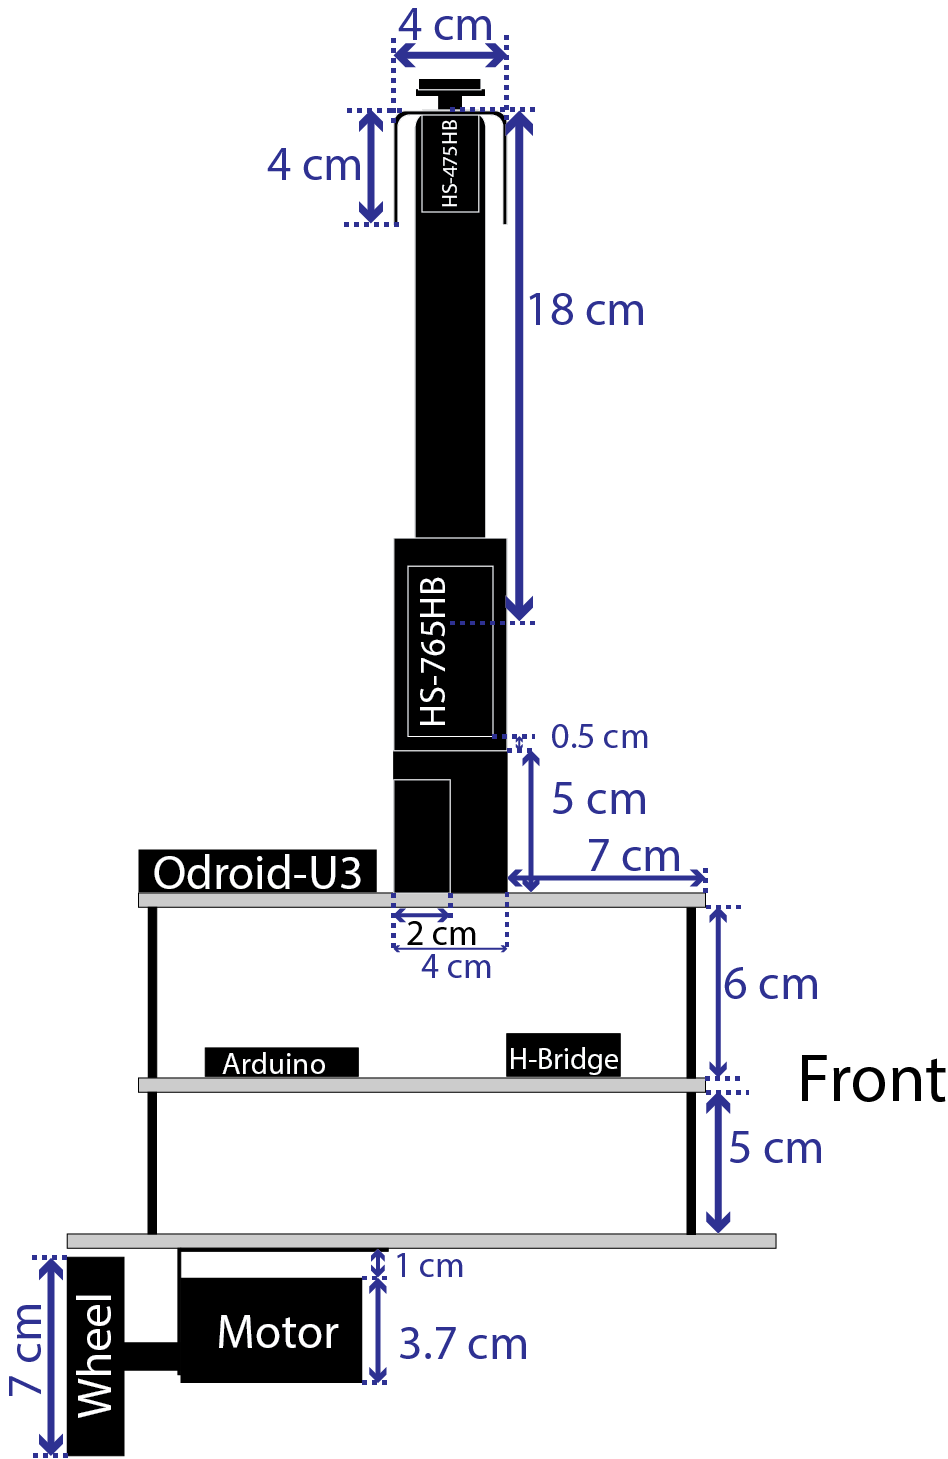
\includegraphics[width=\textwidth]{./Images/upperFourthD.png}
	\caption{Triskarino design.}
	\label{fig:design}
	\end{subfigure}
	\begin{subfigure}[c]{0.2\textwidth}
	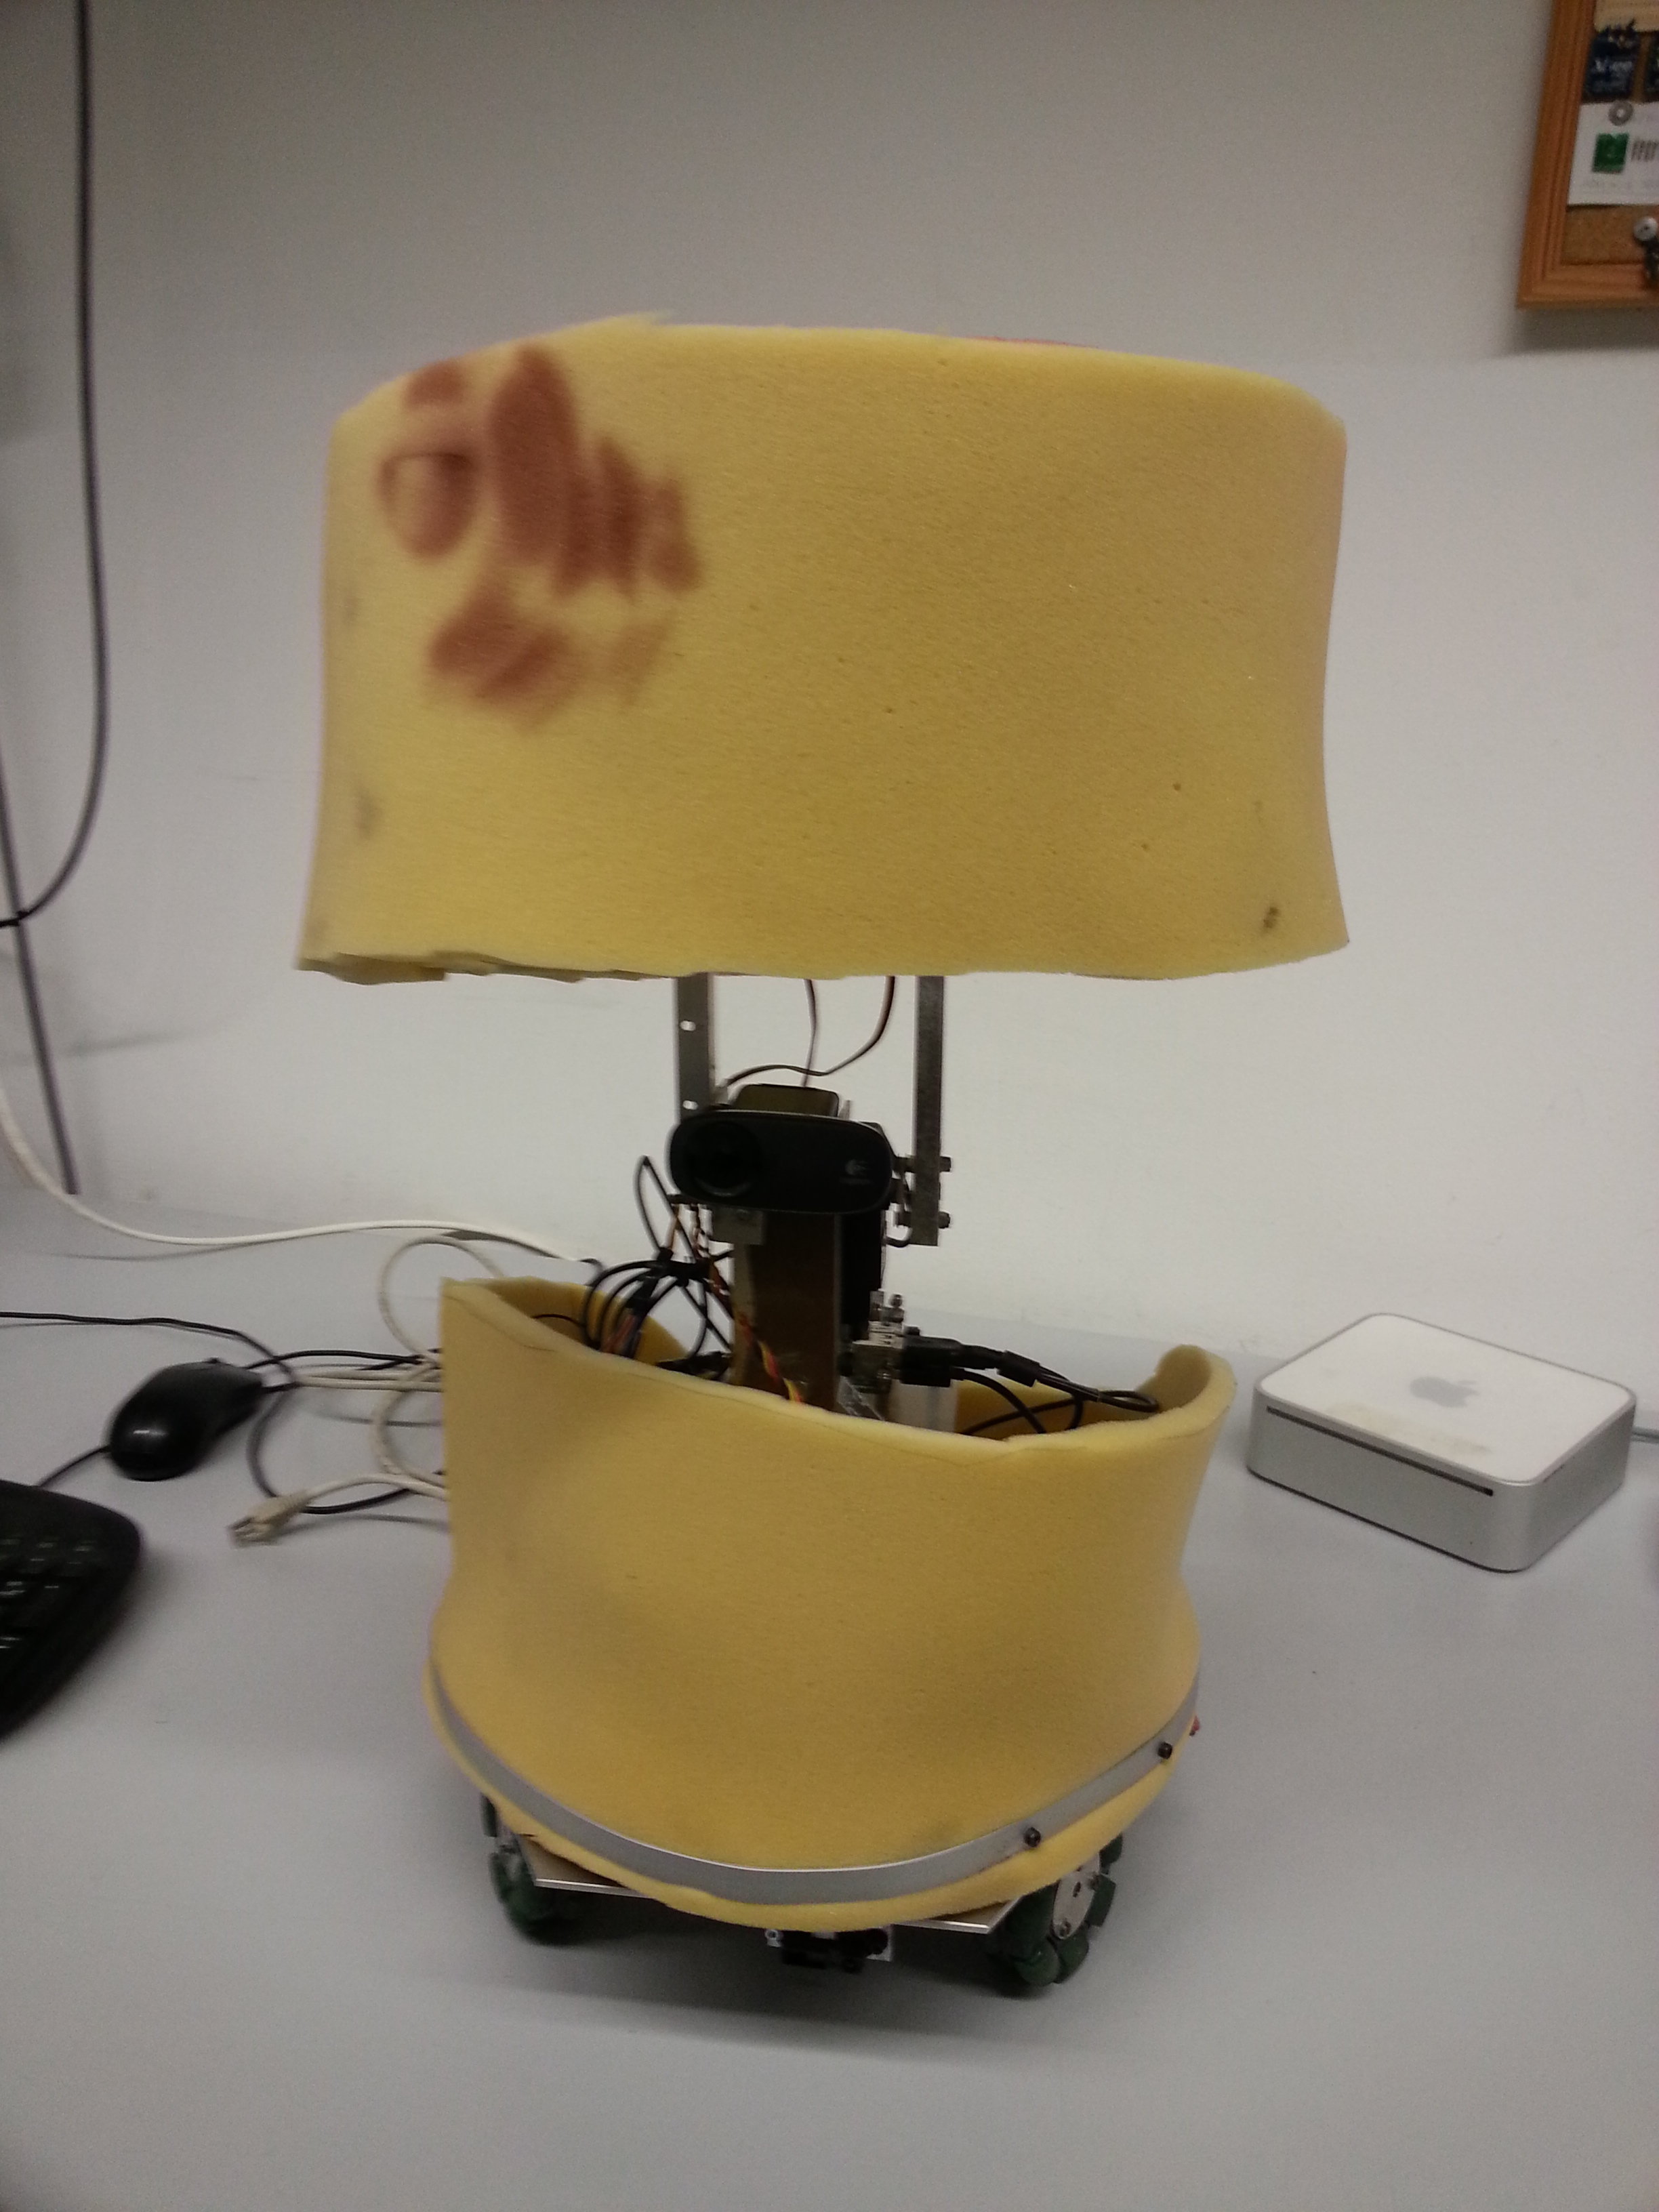
\includegraphics[width=\textwidth]{./Images/platform_fome.jpg}
	\caption{Triskarino with its cover.}
	\label{fig:triskar}
	\end{subfigure}
	\caption{Triskarino platform.}
	\label{fig:robot}
\end{figure}  
 During these studies the system was just used to move the robot in straight line with different emotions, each one selected from our command console. But to show the whole capabilities of the emotional enrichment system and the approach used by us, it was described a little scene that we are preparing. The scene is a modification of the first part of the balcony scene of Shakespeare's Romeo and Juliet play~\cite{RAndJ}. The simplified sketch of our version could be seen in the Fig.~\ref{fig:triskar_test}. As it can be seen the stage was divided in 81 squares and the positions were given to the system in term on the desire square, which allow the robot to adjust to the stage's dimension. The whole sequence of actions were specified as unique action, having several sequential context and just move body action. The other actions, such oscillate body or blend upper body were added online accordingly the desired emotion.  
\begin{figure}
	\centering
	%\begin{subfigure}[c]{0.2\textwidth}
	%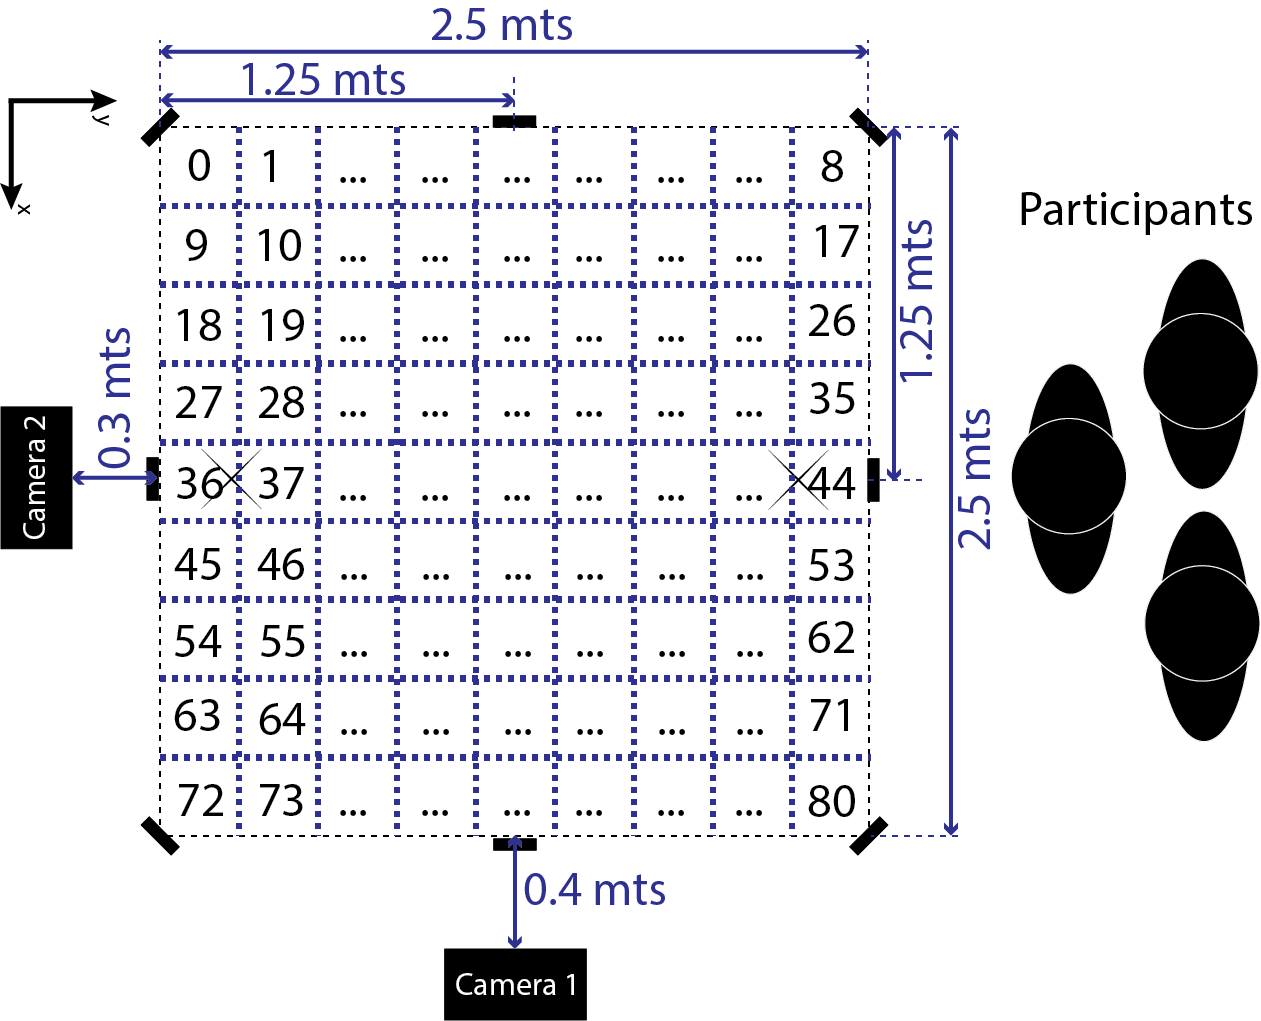
\includegraphics[width=\textwidth]{./Images/FourthCaseScene.png}
	%\caption{Division of the stage.}  
	%\label{fig:design}
	%\end{subfigure}
	%\begin{subfigure}[c]{0.2\textwidth}
	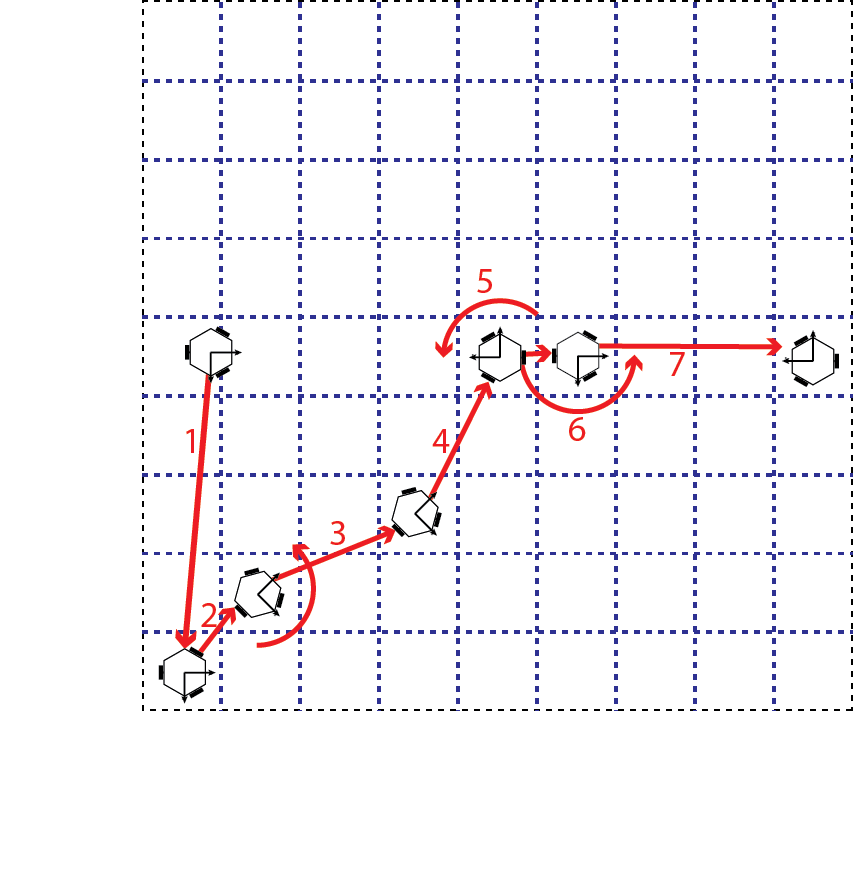
\includegraphics[width=0.4\textwidth]{./Images/FourthCaseSceneB.png}
	%\caption{Movements.}
	%\label{fig:triskar}
	%\end{subfigure}
	\caption{Sketch of Romeo's movements for the balcony scene in Romeo and Juliet play. The arrows show the direction of the movements, and the numbers their sequence.}
	\label{fig:triskar_test}
\end{figure} 
%The sequence of movements done by the robot could be seen in Fig.~\ref{fig:triskar_movements} and in the video. As it could be seen the robot  and they were selected and executed autonomously by the system.
%\begin{figure*}
%	\centering
%	\includegraphics[width=1.0\textwidth]{Images/Sequence_Triskar.png} 
%	\caption{The actual movements of Triskarino in the Balcony scene.}
%	\label{fig:triskar_movements}
%\end{figure*}